\noindent Apart from examining the distributions of blood flow and haematocrit in microvascular networks, it is also important to understand the effects of blood flow properties on the flow resistance of each microvessel within the microvascular networks. To describe the behaviours of non-Newtonian blood flow in the networks of microvessels, apparent viscosity ($\mu_{app}$) is commonly used given the fact that non-continuum effects are dominant at the micro-scale. For this reason, Pries Viscosity Models\cite{Pries1992BloodHematocrit, PriesAR1994RtBF} (Equations \ref{viscosity_equation4}$-$\ref{viscosity_equation2}) were used calculated the empirical predictions to compare with the evaluated $\mu_{app}$ from simulation data (via Poiseuille's Law). On top of this, a comparison of $\mu_{app}$ calculations based on D$_{G}$ and D$_{H}$ was conducted to evaluate which diameter was the preferable input parameter for $\mu_{app}$ estimation. Also, it should be pointed out that Poiseuille’s law was primarily used to work out the apparent viscosity of blood as if it is a constant variable. However, this is actually not true in view of the fact that blood viscosity varies against shear rates and this is known as the shear-thinning effect.\cite{YELESWARAPU1998257, yeleswarapu1998evaluation, BodnarT2011Sott}


\begin{figure}[H]
\centering
\begin{subfigure}{0.48 \textwidth}
    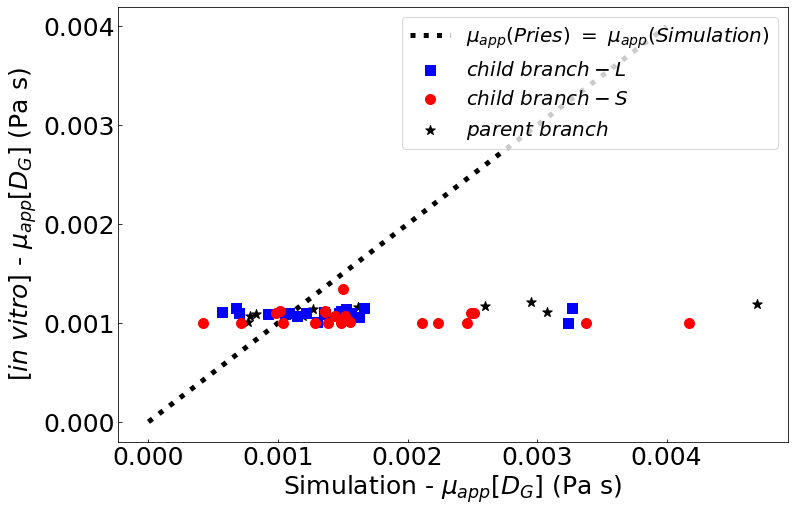
\includegraphics[width=1\textwidth]{images/InVitroApparentViscosityDG.png}
    \caption{\textit{} \label{InVitroApparentViscosityDG}}
\end{subfigure}
\hfill
\begin{subfigure}{0.48 \textwidth}
    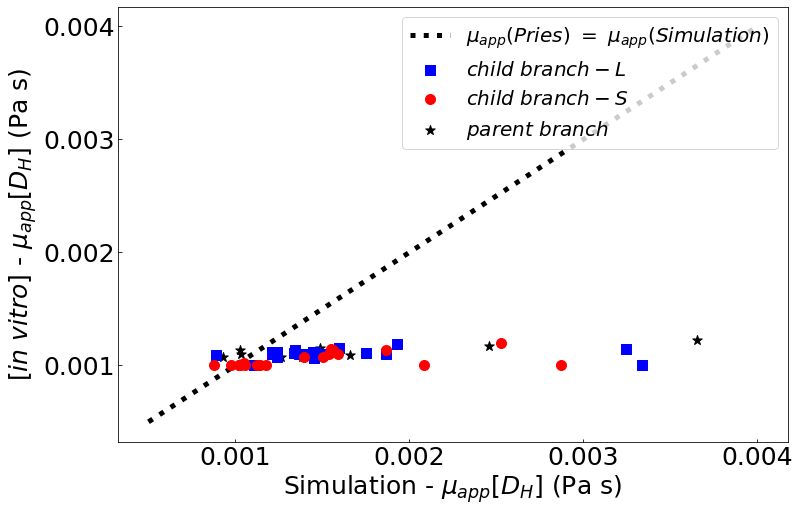
\includegraphics[width=1\textwidth]{images/InVitroApparentViscosityDH.png}
    \caption{\textit{} \label{InVitroApparentViscosityDH}}
\end{subfigure}
\begin{subfigure}{0.48 \textwidth}
    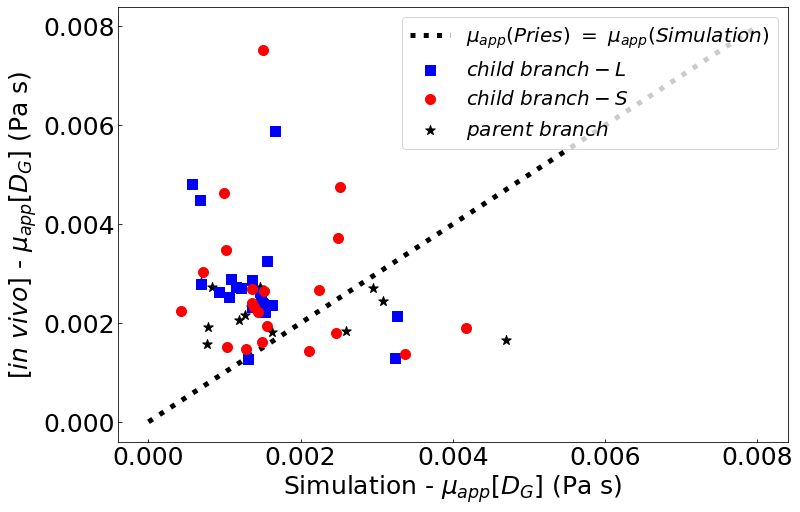
\includegraphics[width=1\textwidth]{images/InVivoApparentViscosityDG.png}
    \caption{\textit{} \label{InVivoApparentViscosityDG}}
\end{subfigure}
\hfill
\begin{subfigure}{0.48 \textwidth}
    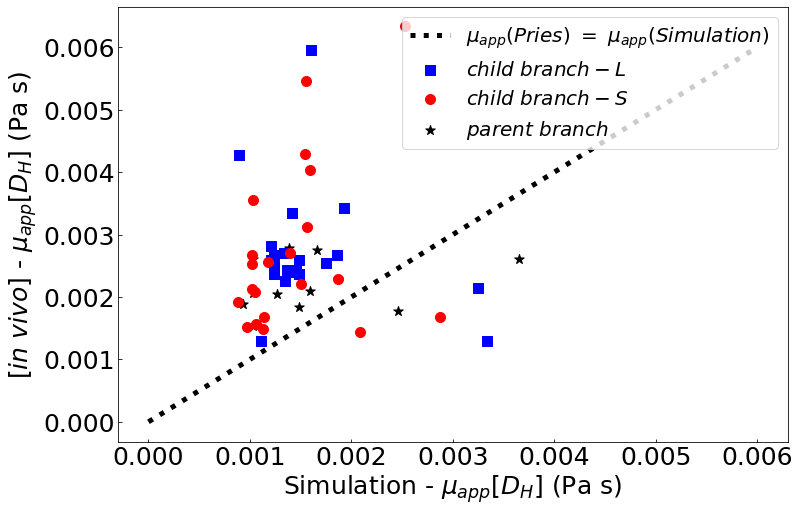
\includegraphics[width=1\textwidth]{images/InVivoApparentViscosityDH.png}
    \caption{\textit{} \label{InVivoApparentViscosityDH}}
\end{subfigure}
\caption{\textit{Comparison of simulation data against empirical predictions from Pries Viscosity Models based on both D$_{G}$ and D$_{H}$. (a$-$b) are for \textit{in vitro} and (c$-$d) for \textit{in vivo}. The "L"/"S" indicate the relatively larger (blue squares) and smaller (red circles) child branches in each diverging bifurcation respectively. The black dotted line represents when the empirical predictions and simulation data are equivalent.} \label{PriesViscosityModels}}
\end{figure}


\noindent Considering the simulation data as our reference data to test the Pries Viscosity Models, the majority of the empirical predictions from \textit{in vitro} formulation were found to be smaller than simulation data for both D$_{G}$ and D$_{H}$. This indicates that the empirical predictions from \textit{in vitro} formulation are underestimating the simulation data (Figure \ref{PriesViscosityModels}a$-$b). The primary reason for this observation is due to the irregular inner vessels that contour across the studied microvascular networks while the \textit{in vitro} empirical model was derived using long and straight glass capillary tubes. Unlike the \textit{in vitro} formulation, majority of the empirical predictions from \textit{in vivo} formulation are overestimating the simulation data (Figure \ref{PriesViscosityModels}c$-$d). This was expected because the simulation data does not consider the presence of endothelial surface layer and the nano-structured glycocalyx in contrast to the \textit{in vivo} formulation of Pries Viscosity Model.\cite{PriesAR1994RtBF} Evidence in support of this was shown in previous studies\cite{LIPOWSKY1977345, LIPOWSKY1980297, SECOMB2013470, PriesAR1994RtBF} where $\mu_{app}$ values were indeed substantially higher in microvessels than in corresponding glass tubes due to the presence of endothelial surface layer. 


\begin{table}[H]
\centering
\caption{\textit{Overall average errors of empirical prediction by Pries Viscosity Models (\textit{in vivo} \& \textit{in vitro}) in comparison to simulation data. The coloured numbers (red and green) indicate the relatively larger and smaller deviations respectively.}
\label{AdoptionOfDHoverDG}}
\scalebox{1}{
\begin{tabular}{*{5}{c}}
\dtoprule
\multirow{2}{*}{\textbf{Average Error $\%$}} & \multicolumn{2}{c}{\textbf{Pries (\textit{in vivo})}} & \multicolumn{2}{c}{\textbf{Pries (\textit{in vitro})}} \\
\cmidrule(lr){2-3} \cmidrule(lr){4-5}
& D$_{G}$ & D$_{H}$ & D$_{G}$ & D$_{H}$ \\
\midrule[0.5pt]
Larger CBs & \textcolor{red}{56.75} & \textcolor{mygreen}{51.66} & \textcolor{red}{45.45} & \textcolor{mygreen}{44.8} \\
Smaller CBs & \textcolor{red}{53.08} & \textcolor{mygreen}{49.9} & \textcolor{red}{76.2} & \textcolor{mygreen}{36.95} \\
PBs & \textcolor{red}{52.98} & \textcolor{mygreen}{41.6} & \textcolor{red}{58.4} & \textcolor{mygreen}{45.4} \\
\dbottomrule
\end{tabular}}
\end{table}

\noindent Based on the above findings, it implies that the simulation data appears to be in-between the predictions from these two empirical models and D$_{H}$ was found to be outperforming D$_{G}$ since both empirical models (\textit{in vivo} \& \textit{in vitro}) gave closer predictions. (see Table \ref{AdoptionOfDHoverDG} for complete error evaluation) Furthermore, the largest average error between the \textit{in vivo} formulation and simulation data for D$_{H}$ was found to be the larger child branches. Therefore, this points out that Pries Viscosity Model (\textit{in vivo}) becomes invalid for smaller child branches at bifurcations. 


\begin{figure}[H]
\centering
\begin{subfigure}{0.48 \textwidth}
    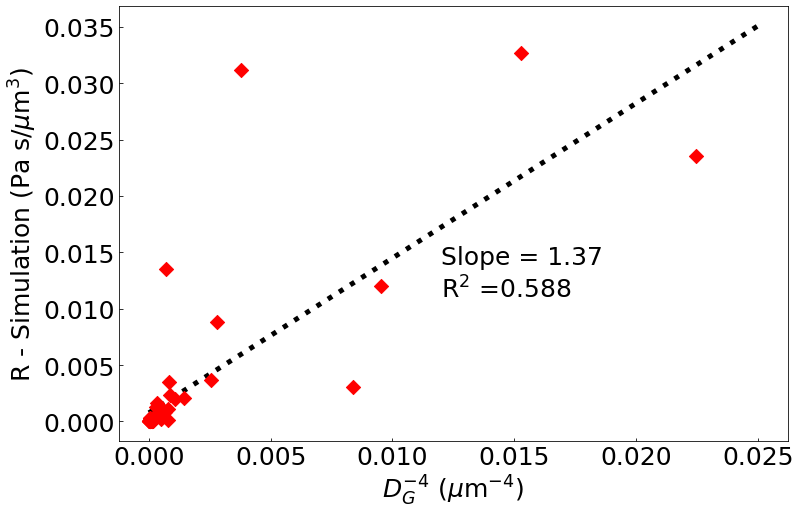
\includegraphics[width=1\textwidth]{images/PoiseuilleR_DG.png}
    \caption{\textit{} \label{PoiseuilleR_DG}}
\end{subfigure}
\hfill
\begin{subfigure}{0.48 \textwidth}
    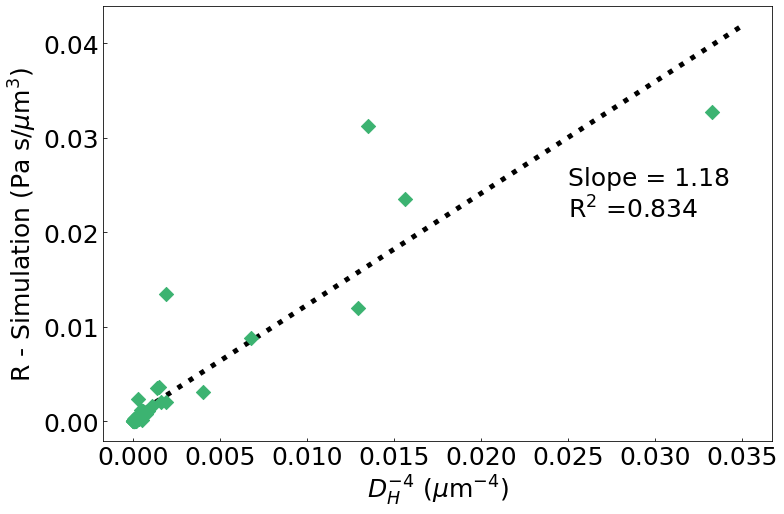
\includegraphics[width=1\textwidth]{images/PoiseuilleR_DH.png}
    \caption{\textit{} \label{PoiseuilleR_DH}}
\end{subfigure}
\caption{\textit{Correlation between flow resistance and branch diameters (D$_{G}$ \& D$_{H}$) from simulation data, including gradient and R-square values of best-fit linear lines.} \label{PoiseuilleRDs}}
\end{figure}

\noindent To further valid the adoption of D$_{H}$ over D$_{G}$, the evaluated flow resistance from simulation data was plotted as a function of D$^{-4}$ to observe how the use of D$_{H}$ in replace of D$_{G}$ contributes to a better approximation of the simulation data with Poiseuille's law. A best-fitted line was included for both diameters to obtain the R-squared value (R$^{2}$) of the fitting line as this value reflects how well the linear line captures the data distribution. From Figure \ref{PoiseuilleRDs}, the evaluated R$^{2}$ values for both D$_{G}$ and D$_{H}$ are 0.588 and 0.834 respectively. These values indicate that only 58.8\% of the residual variance of flow resistance from simulation can be explained by Poiseuille's law for D$_{G}$ whereas it is 83.4\% for D$_{H}$. Therefore, this does suggest that D$_{H}$ is indeed the preferred input parameter for $\mu_{app}$ estimation compared to D$_{G}$. As a result, the following $\mu_{app}$ estimations mentioned below will all be premised on D$_{H}$. 